\chapter{DTM Hardware}

\textbf{This chapter borrows heavily from the DEAP-3600 Electronics $\&$ \gls{daq} Technical Design Report \cite{technicalReport}\footnote{\url{https://www.snolab.ca/deap/private/TWiki/bin/view/Main/TechnicalDesignReport}}}
\begin{description}
\item[EDEV Project Location: ]\url{https://edev.triumf.ca/project/deap/edevel00013}
\end{description}
The \gls{deap3} Digitizer and Trigger Module (\gls{dtm}) is a custom built 6U \gls{vme} motherboard populated with three daughter mezzanine boards (shown in Fig. \ref{Fig:DTM} and schematically in Fig. \ref{Fig:daqSystemCartoon}) (designed by the TRIUMF EDEV department). 
The main motherboard has three \gls{fpga} Mezzanine Card (\gls{fmc})\footnote{See Samtec for data sheets and the standard description: \url{https://www.samtec.com/standards/fmc}} standard connectors which each interface with the daughter boards through a Xilinx Spartan-6 LX \gls{fpga}.
The motherboard is equipped with an Altera Stratix IV GX \gls{fpga}\footnote{\url{https://www.altera.com/products/fpga/stratix-series/stratix-iv/overview.html}} which is used as the primary processing and communication driver for the \gls{dtm}. It is this primary \gls{fpga} that the triggering firmware is implemented on (see Chapter \ref{chap:triggers} for the trigger descriptions).

The \gls{dtm} receives 22 analog sums (\gls{asum}s) of 12 \gls{pmt} signals from the signal conditioning boards (\gls{scb}s) which are digitized by the ADC mezzanine board (Section \ref{sec:adcBoard}). The \gls{dtm} is constantly integrating the \gls{asum}s and uses \gls{fprompt} and charge to make a triggering decision. If the triggering requirements are met (as discussed in Chapter \ref{chap:triggers}) the \gls{dtm} will send a trigger command through the I/O board (Section \ref{sec:nimBoard}) to the first in a chain of digitizers which passes the trigger along to the rest in a daisy-chain arrangement (see Fig. \ref{Fig:triggerDist}).

Two mezzanine board configurations have been used and are discussed in Section \ref{sec:dtmConfigs}. The four types of mezzanine boards used are discussed in this chapter, information pertaining to their associated firmware releases can be found in Chapter \ref{chap:firmware}. 

\begin{figure}[ht]
\centering
\includegraphics[height = 0.4\paperheight]{3xFMC_imageTOP}
\caption{The digitizer and trigger module motherboard. The three \gls{fmc} slots are labelled to the left of the board. Digital control is implemented on an Altera Stratix IV GX FPGA while interfacing with the \gls{fmc}s are controlled by the three Spartan-6 FPGAs.}
\label{Fig:DTM}
\end{figure}


%\begin{figure}[ht]
%\centering
%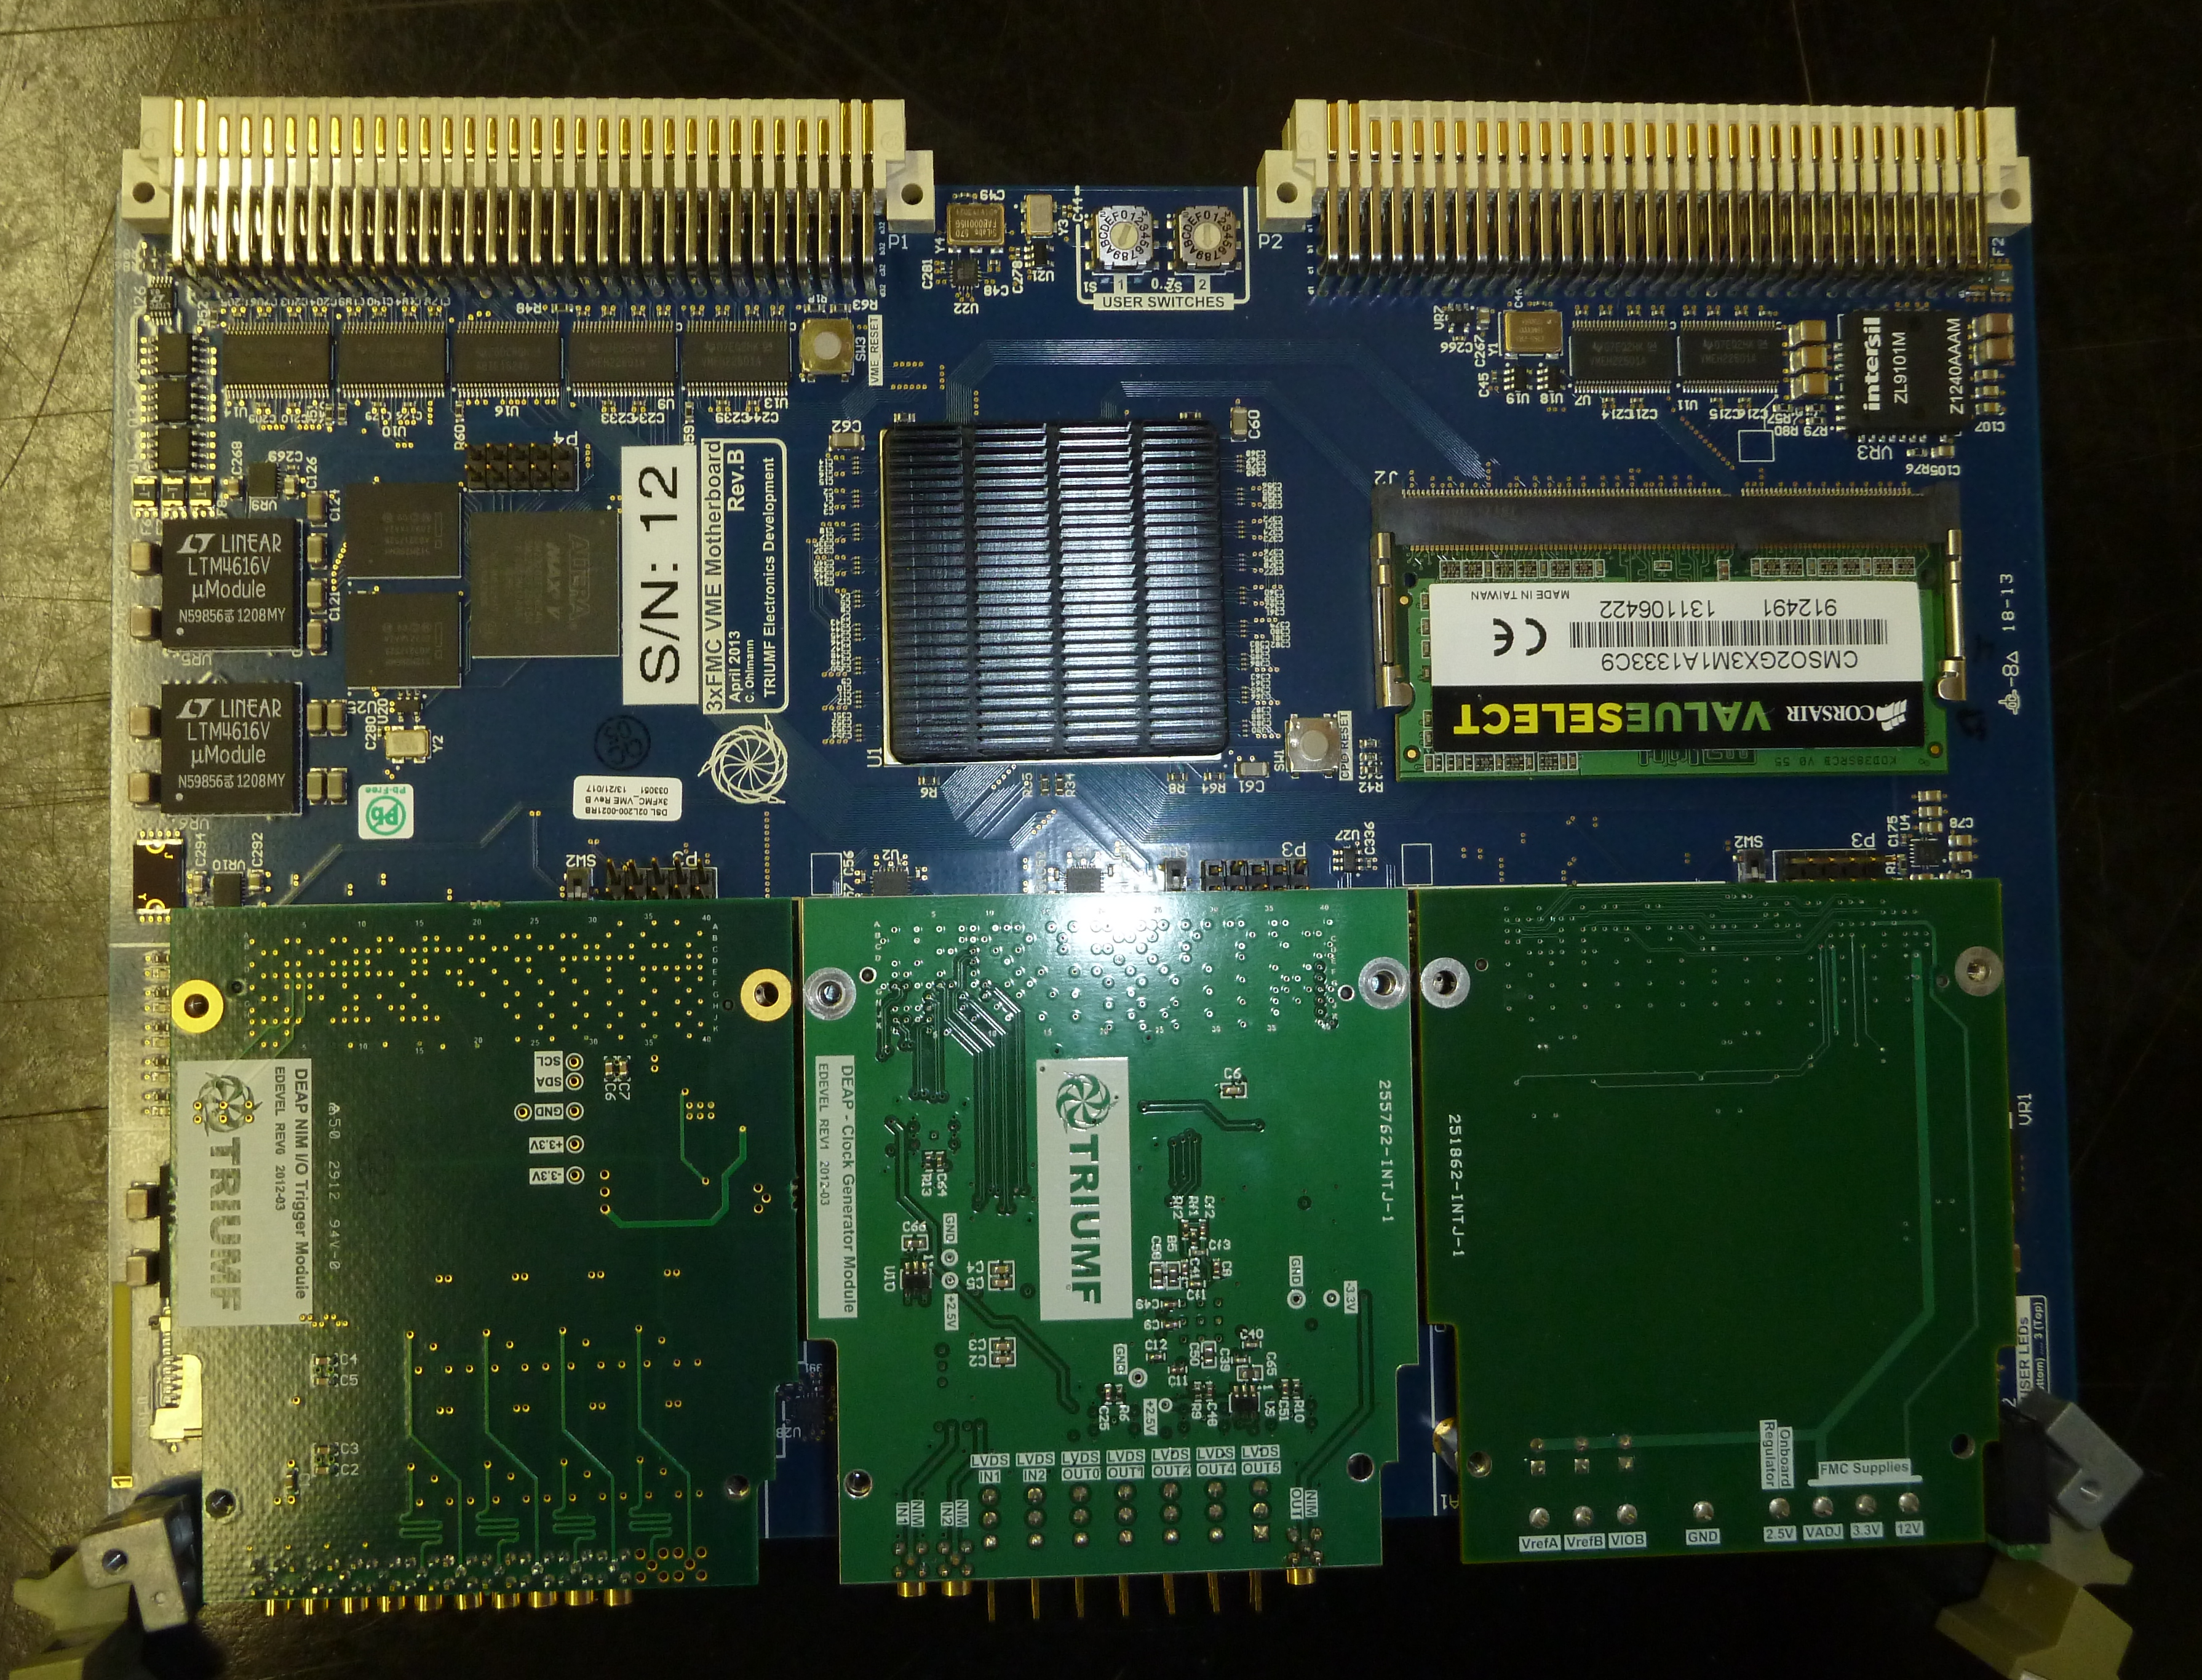
\includegraphics[height = 0.4\paperheight]{DTMModule}
%\caption{The digitizer and trigger module populated with the ADC, trigger I/O, and the clock mezzanine boards. Digital control is implemented on an Altera Stratix IV GX field programmable gate array.}
%\label{Fig:DTM}
%\end{figure}

\begin{figure}[ht]
\centering
\includegraphics[width = 0.85\paperwidth]{daqSystemCartoon}
\caption{Diagram of the information and signal flow in the \gls{dtm}. The clock generator mezzanine board is shown as being used although this is subject to change (see Section \ref{sec:dtmConfigs} for more on the configurations)}
\label{Fig:daqSystemCartoon}
\end{figure}


\section{VME 3xFMC Carrier Motherboard}
\begin{description}
\item[EDEV Project Location: ]\url{https://edev.triumf.ca/svn/edevel00052}
\end{description}
Most modern experiments have many common characteristics when it comes to data acquisition, processing, and triggering. These mixed signal systems typically use some combination of fast ADC’s and general purpose I/O to capture and digitize any relevant data which is then piped into an \gls{fpga} for processing. Various data suppression algorithms and triggering schemes are implemented before the final events of interest are displayed or written to disk.
Large memory buffers are often necessary to prevent data loss and maximize the rate at which data can be acquired without overloading the processing capabilities of the \gls{fpga} or associated communication channels. The \gls{vme} 3x\gls{fmc} motherboard was conceived as a way to make better use of development resources. It was designed to meet these general needs while providing the flexibility to rapidly adapt to more specific project requirements.


An Altera Stratix IV GX \gls{fpga} (EP4SGX230KF40C2N)\footnote{\url{https://www.altera.com/products/fpga/stratix-series/stratix-iv/overview.html}} serves as the main processing and communication hub for the motherboard module. The \gls{vme} interface for the motherboard is provided by the Stratix IV GX \gls{fpga}. With the correct firmware, the motherboard fully supports all \gls{vme} data and addressing modes and may be implemented as most types of \gls{vme} module (Master, Slave, Arbiter, etc.). To support high speed ADCs and back-end communications (outside of \gls{vme}), this \gls{fpga} has 28 dedicated gigabit serial links going to the \gls{fmc} mezzanines (10, 10, and 8). Each link is capable of operating at data rates up to 8.5 Gbps.


Additional Xilinx Spartan-6 LX \gls{fpga}s (XC6SLX45-2FGG484I)\footnote{\url{http://www.xilinx.com/support/documentation/data_sheets/ds160.pdf}} are used for each of the three \gls{fmc}s providing support for bidirectional differential signalling (required by the \gls{fmc} specification).
The bidirectional differential signalling allows maximum compatibility for both custom and commercially available \gls{fmc} modules. 
Each \gls{fmc} interface on the carrier motherboard supports both single ended and differential I/O on banks LA and HA (except HA23), and single ended I/O and input only differential on bank HB (and HA23). 
This configuration gives a maximum per \gls{fmc} of 80 differential pairs (23 input only), 160 single ended I/O, or any combination thereof. 
Although the Spartan-6 LX \gls{fpga}s are mainly used for I/O interfacing, they also provide resources for additional data buffering, delay matching, and additional processing power. 

The carrier motherboard provides a very flexible clocking scheme. The \gls{vme} interface also provides a 16 MHz system clock.
On board oscillators provide fixed 16 MHz and 500 MHz clocks while a programmable oscillator (defaulting to 125 MHz) allows additional flexibility and a dedicated DDR3 memory interface reference clock. 
Each \gls{fmc} module may provide up to two dedicated gigabit transceiver reference clocks and two dedicated clock inputs which allow the option for mezzanine mounted oscillators or external clock inputs of any frequency.
All of these clock sources use dedicated \gls{pll} inputs on the Stratix IV GX and may be multiplied to any synthesizable frequency for driving internal logic or a wide variety of clock outputs.


To meet the data buffering and general computing memory requirements, the motherboard includes a 204 pin DDR3 SO-DIMM interface (laptop memory). 
The memory controller on the Stratix can supports up to 2 GB with a memory clock up to 533 MHz. 
This translates into a peak transfer rate of approximately 8.5 GB/s. For configuration management, an Altera MaxV CPLD (5M2210ZF256C5N)\footnote{\url{https://www.altera.com/content/dam/altera-www/global/en_US/pdfs/literature/hb/max-v/max5_handbook.pdf}} and 1Gb (2 x 512 Mb) of NOR flash memory is provided. The flash memory is directly accessible from the Stratix to allow for self programming and reconfiguration through \gls{vme} or other communication interfaces.
Uncompressed bitstreams for the Stratix IV GX and Spartan-6 \gls{fpga}s are 94,557,472 and 11,939,296 bits respectively so the provided flash allows support for several configurations for each with enough left over for some user data. 
While the CPLD handles the configuration of the Stratix, the configuration of the Spartan-6 \gls{fmc} interface \gls{fpga}s is managed by the main Stratix IV GX \gls{fpga}. This scheme allows for \gls{fmc} module identification and consequent reprogramming of the interface \gls{fpga}s.


Power management on the motherboard has also been implemented to allow maximum flexibility. The power design supports use in \gls{vme} crates with or without the 3.3V supply provisioned in the VME64X spec\footnote{For the standard see: \url{http://file.wiener-d.com/documentation/General/WIENER_VME_VXI_VXS_introduction_1.0.pdf}}. 
While all supply voltages are provided regardless of the crate used, additional power is available for the individual \gls{fmc} modules when the 3.3V supply is present. 
Each \gls{fmc} slot is supplied with a 12V ($<$1A) and 3.3V ($<$3A) fixed supplies and a dedicated 0-3.3V adjustable supply, VADJ ($<$4A). 
In return, the \gls{fmc} modules provide the carrier with I/O voltage for bank B and reference voltage for banks A and B if voltage referenced I/O standards are used.
All of the power supplies are monitored and controlled from the Stratix IV GX \gls{fpga} on the carrier motherboard.


The \gls{vme} 3x\gls{fmc} Carrier Motherboard is a very flexible and capable card, however, most of the actual functionality comes from the \gls{fmc} modules that are physically plugged in whether custom built or commercially available.



\subsection{Motherboard Components}
The major components of the \gls{dtm} consist of the following:

\begin{description}
	\item[(1) Altera Max V CPLD] \hfill \\
	On power-up configures the Stratix IV FPGA, and allows JTAG programming of both the Stratix IV and the Flash memory. Also performs watchdog on Stratix IV.
	
	\item[(1) Altera Stratix IV FPGA] \hfill \\
	Core of the \gls{dtm}. Performs \gls{vme} transfers, runs NIOSII embedded processors, trigger system, and configures the Spartan-6s. Only \gls{fpga} with direct access to DDR3 SDRAM, LEDs, switches, and \gls{vme}. Shares bus to Flash memory with Max V.
	
	\item[(1) DDR3 SDRAM DIMM] \hfill \\
	Used for ADC data storage
	
	\item[(2) 512 Mb Flash Memory Chips] \hfill \\ 
	Contain configuration files for Stratix IV and Spartan-6 FPGAs. 
	
	\item[(3) Xilinx Spartan-6 LX FPGAs] \hfill \\
	Used to decode ADC, initialize the clock module, and connect the FMCs I/O to the Stratix IV.
	
	\item[(3) FMC connectors] \hfill \\ 
	Where the mezzanine cards go.
	
	\item[(9) User-controlled LEDs] \hfill \\ 
	Diagnostics and status
	
	\item[(2) User-controlled 16 position switches] \hfill \\ 
	Set VME address of DTM
	
	\item[(1) VME64 compatible backplane] \hfill \\ 
	Communication link of DTM
\end{description}


\subsection{Board Revisions}

There have been two revisions of this motherboard to date, Rev.A and Rev.B\footnote{See the errata for firmware compatibility issues (Chapter \ref{chap:errata})}. The primary difference between these revisions is only the addition of a SD card on Rev.B. Although the hardware is essentially identical there were issues that arose which meant that the firmware release edevel00268 only worked on Rev.B boards although this issue has been fixed in the newer edevel00365 releases and the boards can now be used interchangeably (See Chapter \ref{chap:firmware} and \ref{chap:errata}).

\subsection{Board Settings $\&$ Registers}
\subsubsection{VME Address}
\begin{description}
\item[Twiki Location: ]\url{https://www.snolab.ca/deap/private/TWiki/bin/view/Main/Dtmboard}
\end{description}
The motherboard is equipped with two rotary switches for setting the \gls{vme} base address. Default setting is 0x69 = sw2[7-4]: 0110, sw1[3-0]: 1001. \textbf{Bit 0}, the boot bit, \textbf{must always be on}. Bit[7-4][3-0] $\rightarrow$ 0110 1001 $\rightarrow$ 0xB(3,7-5) corresponding to the upper 4 bits of the A24: 0xB00000 (Rotary switch: 0x69), bit[7-4][3-0] $\rightarrow$ 1000 1001 $\rightarrow$ 0xC(3,7..5) corresponding to the upper 4 bits of the A24: 0xC00000 (Rotary switch: 0xC9).

The \gls{vme} base address has to be adjusted correspondingly in the frontend or access code (deap/pro/FrontEnd/dtm/vme\_register.h (DTM\_BASE)). No two \gls{vme} modules being used can use the same base address. %\footnote{See the errata for base address changes (Section \ref{sec:baseAddressErrata})}. 

\subsubsection{DTM Registers}
\begin{description}
\item[Twiki Location: ]\url{https://www.snolab.ca/deap/private/TWiki/bin/view/Main/Dtmregisters}
\end{description}

In general, there exist two type of registers: ReadWrite (RW) and ReadOnly (RO). The first type is used to set parameters through \gls{odb} (see Section \ref{sec:odb}), the second one to read the status and data of the different \gls{dtm} firmware modules. The last two bits of the address are not used, therefore the distance between registers is 0x4 in address space.

The exact register address is given by:

DTM\_BASE + (RW/RO/USER)\_OFFSET + REG\_OFFSET

Reading of these registers can be done over \gls{jalisco} (see Section \ref{sec:jalisco}) or using \gls{vme} command line commands using vme\_read.exe -b 0xb00000 (which is the dtm base) -a (register address)\footnote{See the twiki for how to run this:\\ \url{https://www.snolab.ca/deap/private/TWiki/bin/view/Main/UsingTriumfDtmTestSetup}}.

\NOTE{The registers in \gls{jalisco} are displayed in 32 bit words, so the \gls{jalisco} offset is the register table offset/4.}

\section{Mezzanine Boards $\&$ DTM Connections}
The following describes the different \gls{fmc} boards used and connections in the various \gls{dtm} configurations. The different configurations themselves are discussed in Section \ref{sec:dtmConfigs} with their associated firmware in Chapter \ref{chap:firmware}.

\subsection{24 Channel ADC FMC}
\label{sec:adcBoard}
\begin{description}
\item[SVN Project Location: ]\url{https://edev.triumf.ca/svn/edevel00018}
\item[SVN Firmware Location: ]\url{https://edev.triumf.ca/svn/edevel00230}
\item[Hardware Connections: ]\url{https://www.snolab.ca/deap/private/TWiki/bin/view/Main/HWconnection#FMCADC}
\end{description}
The ADC (or Digitizer) board, seen in Fig. \ref{Fig:adcBoard} is populated with three eight channel 12-bit 45 \gls{msps} $\Sigma - \Delta$ ADCs (ADC12EU050)\footnote{Data sheet: \url{http://www.ti.com/lit/ds/symlink/adc12eu050.pdf}}. 
The \gls{dtm} receives 22 analog sums (\gls{asum}s) of 12 \gls{pmt} signals from the \gls{scb}s which are digitized by the ADC mezzanine board\footnote{Have a look at the \gls{deap3} technical manual or the \gls{deap} electronics paper}. These digitized \gls{asum}s are used to make the trigger decision as discussed in Chapter \ref{chap:triggers}. 

The \gls{scb} \gls{asum} output signals are received on differential lines by the ADC. The differential common mode is 0.6 V.
To match the ADC $\pm$1.05 V dynamic range the \gls{scb} applies a constant offset of 0.8 V to the \gls{asum} signal.
The ADC are supplied a 45.161290 MHz clock by a \gls{pll} on the \gls{dtm}\footnote{Other documentation reports a 50 MHz clock to the ADCs, that is out of date. This is the maximum allowed speed of the ADCs.}.

\NOTE{The PLL is set to 45.25 MHz but the 45.161290 MHz is the fastest it can run, hence the odd rate.}

To ensure a low jitter clock for sampling and data transfer off the ADC, this clock is first passed through a clean-up \gls{pll} integrated into the ADC. 
The 12-bit data sampled by the ADC at 45.161290 MHz is transferred to the Spartan-6 \gls{fpga} as serial DDR data.% at 350 MHz along with a corresponding 350 MHz bit clock \FIXME{IS THIS RATE CORRECT?}.
To enable the correct re-alignment of the 12-bit data word in the \gls{fpga} a word clock is also provided by the ADC. Control of the ADC is performed via a serial to parallel interface (SPI) command protocol.
To test data alignment the ADC provides default test patterns and a user defined test pattern. The test patterns are enabled and in the case of the user test pattern defined over the SPI command structure.
\gls{jalisco} includes tools for reading and debugging ADC's, refer to Section \ref{sec:jalisco}.

\textbf{Configuration Notes:} Unchanged board used in all configurations of the \gls{dtm} and for firmware modules edevel00268 and edevel00365.

\begin{figure}
\centering
\includegraphics[width = .5\textwidth]{adcBoard}
\caption{24 Channel digitizer board which receives 22 analog sums of 12 \gls{pmt}s each and passes the digitized result to the main Stratix IV \gls{fpga} for a trigger decision to be made.}
\label{Fig:adcBoard}
\end{figure}


\subsection{DEAP Clock Generator Module}
\label{sec:mClockBoard}
\begin{description}
\item[SVN Project Location: ]\url{https://edev.triumf.ca/svn/edevel00114}

\item[SVN Firmware Location: ]\url{https://edev.triumf.ca/svn/edevel00230}

\item[Hardware Connections: ]\url{https://www.snolab.ca/deap/private/TWiki/bin/view/Main/HWconnection#FMCCLOCK}
\end{description}

The clock generator board distributes an 62.5 MHz clock generated in the Stratix IV to the rest of the \gls{daq} system via a daisy chain arrangement. These are distributed as: four clock signals to the four \gls{v1720} sectors; one clock signal to the \gls{v1740} sector; and one clock signal to the \gls{ppg} module. The 62.5 MHz clock distribution to the four \gls{v1720} sectors, the \gls{v1740} sector and the \gls{ppg} as discussed in Section \ref{sec:daisyChainClock}.
Within the \gls{v1720} and \gls{v1740} sectors the clock signal is daisy chained module to module (see Section \ref{sec:newClock}).

The clock generator \gls{fmc} has seven \gls{lvds} and three \gls{nim} I/O ports. Five \gls{lvds} are used to connect to each of the four clock groups and the VETO \gls{v1740}s. One \gls{nim} port is used for the \gls{ppg} clock. The remaining ports are unassigned general I/O\footnote{See \url{https://www.snolab.ca/deap/private/TWiki/bin/view/Main/HWconnection}}.

\textbf{Configuration Notes:} Board used in all releases of firmware module edevel00268, replaced with the SFP and Mini-SAS board in mezzanine (See Section \ref{sec:SFPBoard}). Last stable release installed at SNOLAB using this board edevel00268/\tagTwoSixEight. See Section \ref{sec:dtmConfigs} for the different \gls{dtm} configurations, and Section \ref{sec:newClock} for more on the \gls{dtm} and \gls{daq} clocking system.

\begin{figure}
\centering
\includegraphics[width = .5\textwidth]{mClockBoard}
\caption{Seven \gls{lvds} and three \gls{nim} I/O ports configured to provide the master clock to the rest of the \gls{daq} system in a daisy chain clocking configuration (see Section \ref{sec:daisyChainClock}).}
\label{Fig:mClockBoard}
\end{figure}



\subsection{SFP and Mini-SAS Interface}
\label{sec:SFPBoard}
\begin{description}
\item[SVN Project Location: ]\url{https://edev.triumf.ca/svn/edevel00228}
\item[SVN Firmware Location: ]\url{https://edev.triumf.ca/svn/edevel00230}
\end{description}
\noindent This module is equipped with:
	\begin{enumerate}
	\item (1) SFP connector allowing gigabit ethernet
	\item (1) Mini-SAS connector
	\item (1) eSATA connector (can be configured as a clock in)
	\item (1) Micro-SD card
	\end{enumerate}

The SFP and Mini-SAS Interface \gls{fmc} has been designed for the \gls{deap3} experiment to add ethernet networking and data storage on the on-board micro-SD card, see Chapter \ref{chap:install} for interfacing and features.

\begin{figure}
\centering
\includegraphics[width = .5\textwidth]{ethernetBoard}
\caption{SFP ethernet and Mini-SAS interface board which adds FTP readout and flash programming interfacing with the \gls{dtm} (see Chapter \ref{chap:install})}
\label{Fig:ethernetBoard}
\end{figure}


\subsection{DEAP NIM I/O Trigger Module}
\label{sec:nimBoard}
\begin{description}
\item[SVN Project Location: ]\url{https://edev.triumf.ca/svn/edevel00019}
\item[SVN Firmware Location: ]\url{https://edev.triumf.ca/svn/edevel00279}
\item[Hardware Connections: ]\url{https://www.snolab.ca/deap/private/TWiki/bin/view/Main/HWconnection#FMCIO}
\end{description}
The \gls{nim} I/O board is a twelve channel \gls{nim} board used for trigger output, \gls{daq} control/status, calibration systems control, and in one configuration a master clock output\footnote{See the configuration notes and Section \ref{sec:dtmConfigs}}. 

The twelve channels are split between eight dedicated outputs and four dedicated inputs.
The \gls{v1720} and \gls{v1740} can both accept \gls{nim} or TTL logic \cite{v1720UM}\cite{v1740UM}, for compatibility with the \gls{ppg}\cite{ppg} \gls{nim} logic is chosen.
The \gls{v1720} and \gls{v1740} boards specify \gls{nim} lemo-00 50$\Omega$ trigger input connections, the \gls{ppg}\cite{ppg} specifies \gls{nim} lemo-00 inputs.
Due to space limitations the I/O board is populated with mmcx connectors\footnote{These are fragile and very prone to breaking}.

\begin{figure}
\centering
\includegraphics[width = .5\textwidth]{nimBoard.jpg}
\caption{12 Channel \gls{nim} I/O board used for controlling the rest of the \gls{daq} system including the output of the trigger signal and busy inputs. In one \gls{dtm} configuration this board also outputs the master clock (see Section \ref{sec:dtmConfigs}).}
\label{Fig:nimBoard}
\end{figure}

\subsubsection{Trigger Distribution}
On the generation of a trigger signal by the \gls{dtm}, or an external trigger input, a trigger signal is distributed to the \gls{daq} system through the \gls{nim} board. 
The trigger signal is distributed on five dedicated trigger lines to the \gls{v1720} and \gls{v1740} sectors.
For the purposes of clock and trigger distribution, the \gls{v1720} and \gls{v1740} digitizers are grouped into five logical sectors (Fig. \ref{Fig:triggerDist}). 
The 32 \gls{v1720}s are grouped into four sectors where each logical sector contains eight physical modules. 
The \gls{v1740} modules form a single logical trigger and clock sector. 
Each logical trigger sector receives a single trigger signal distributed from the \gls{nim} board. 
The signal is received by the first board in each sector and then daisy chained, board to board, within each sector.


\begin{figure}
\centering
\includegraphics[width = \textwidth]{triggerDist}
\caption{Diagram of the trigger signal distribution in the \gls{daq} system.}
\label{Fig:triggerDist}
\end{figure}

\NOTE{For more on the busy signals, see the \href{https://www.snolab.ca/deap/private/TWiki/bin/view/Main/BusySystem}{Twiki}\footnote{\url{https://www.snolab.ca/deap/private/TWiki/bin/view/Main/BusySystem}}}

\section{Clocking} 
\label{sec:newClock}

Currently\footnote{Using edevel00268 July, 2016} the clock distribution and thereby the synchronization of events for the \gls{dtm} and the \gls{v1720} and \gls{v1740} digitizers is done through a daisy chain arrangement.

The stability of this arrangement has been brought into question as some trigger signals were found to be arriving close to the clock boundary. This is an issue as the \gls{v1720} clock delays are only allowed to be certain values rather than arbitrary precision so the tuning of delays is limited. The issue has not arisen after the clock delays were readjusted. Further issues with the daisy chain clocking is that the cables are flaky. 
To address these potential problems a new clock distribution system has been developed. 
The daisy chained \gls{dtm} generated master clock is to be replaced with a \gls{vme} clock distribution system with the master clock being sourced from the \gls{dtm} via the unused output on the NIM I/O board. The clock distribution modules\footnote{\url{https://edev.triumf.ca/project/edev/vme/edevel00163}}, replace the need for a daisy chain arrangement and thereby removing a potential source of error. The clock generator \gls{fmc} on the \gls{dtm} is to be replaced with a SFP and Mini-SAS \gls{fmc}.

\subsection{Daisy Chain Clocking}
\label{sec:daisyChainClock}
The master clock for the \gls{daq} system is generated from the motherboards 50 MHz source clock. A phase lock loop (\gls{pll}) on the \gls{dtm} sets the frequency to 100 kHz for the periodic trigger (see Section \ref{sec:periodicTrigger}), and 62.5 MHz clock for the \gls{ppg} module and the digitizers. The dedicated clock generator mezzanine board passes the 62.5 MHz clock to the first digitizer in groups of at most six which is then passed along the chain. To match the expected trigger delay introduced by daisy chaining, a 3.57 ns delay is added to the clock daisy chain. The clock delay is configurable within the \gls{v1720} or \gls{v1740} modules as described by the manufacturer\cite{v1720UM}\cite{v1740UM}. 

\begin{figure}
\centering
\includegraphics[height = 0.36\paperheight]{daisyChain}
\caption{Clocking diagram of the data acquisition system under the daisy chain configuration}
\label{Fig:daisyChainClock}
\end{figure}

\subsubsection{Distributed Master Clock}
\label{sec:distributedMasterClock}

Replacing the daisy chain clocking is a distributed system removing the necessity of setting delays in the chain. The distributed system used the Clock Distribution Modules\footnote{\url{https://edev.triumf.ca/project/edev/vme/edevel00163}} (\gls{cdm}) designed by the TRIUMF EDEV department for use on the GRIFFIN project. The 62.5 MHz \gls{daq} master clock is generated in the \gls{dtm} and fed through the NIM I/O \gls{fmc} to the first of three the \gls{cdm}. This first slave \gls{cdm} cleans the clock and outputs two synced, phase locked clocks to two other \gls{cdm}s which then fan out all of the \gls{daq} clocks. As the same wire is used for all connections and the sources are synced and phase locked, there is no need for any programmed delays. 


\begin{figure}
\centering
\includegraphics[height = 0.36\paperheight]{distClock}
\caption{Diagram of the clock distribution system for the data acquisition system using a distributed master clock method, replacing the daisy chain configuration in Fig. \ref{Fig:daisyChainClock}.}
\label{Fig:distClock}
\end{figure}
\clearpage
\subsubsection{Clock Distribution Modules}
\begin{description}
\item[EDEV Project Location:] https://edev.triumf.ca/project/edev/vme/edevel00163
\item[Summary:] 24 channel low jitter \gls{lvds} Clock/Sync generation and fan out module
\end{description}
The clock distribution modules, shown in Fig. \ref{Fig:clockDistMod}, are the essential part of the clock distribution system. Designed for the GRIFFIN experiment by the TRIUMF EDEV department, these boards output a stable and phase locked clock through up to 24 channels. 
\begin{figure}
\centering
\includegraphics[height = 0.36\paperheight]{clockDistMod}
\caption{Clock distribution module to be used for the distributed clocking of the system, supplanting the current (July 2016) \gls{daq} daisy chain method.}
\label{Fig:clockDistMod}
\end{figure}

\section{DTM Configurations}
\label{sec:dtmConfigs}
There are two \gls{fmc} configurations used for the \gls{dtm}, both use the same NIM I/O and 24-channel ADC \gls{fmc}s but switch out the clock generator (Fig. \ref{Fig:dtmConfig268}) with the SFP and Mini-SAS board (Fig. \ref{Fig:dtmConfig365}). This change of boards is due to an intended\footnote{Not yet installed at SNOLAB as of July 2016} change in the clock distribution method from a daisy-chain to a distributed phase-locked clock system (see Section \ref{sec:newClock}). The addition of the SFP connection comes with added ethernet capabilities allowing ethernet data readout to replace the current VME readout system (see Chapter \ref{chap:install} for more on the FTP and ethernet data readout). The firmware project that uses the clock generator module is edevel00268 (Section \ref{sec:268}) and the SFP and Mini-SAS project is edevel00365 (Section \ref{sec:365}).
\begin{figure}
\centering
\includegraphics[height = 0.36\paperheight]{dtmConfigClockBoard}
\caption{DTM configuration using the edevel00268 firmware project (see Section \ref{sec:268}). The master clock is generated by the Stratix IV and fed out to the digitizers and externals through the clock generator module (Section \ref{sec:daisyChainClock}). The master clock is fed out to first in a section of digitizers and is passed along in a daisy chain with delays programmed into the digitizers as described in section \ref{sec:daisyChainClock}.}
\label{Fig:dtmConfig268}
\end{figure}

\begin{figure}
\centering
\includegraphics[height = 0.36\paperheight]{dtmConfigSFPMasterClockOut}
\caption{DTM configuration using the edevel00365 firmware project (see Section \ref{sec:365}). The master clock is generated by the Stratix IV and fed out to the digitizers and externals through the NIM I/O module. The master clock is then sent to a clock distribution module in slave mode which feeds out two cleaned, phase locked, and synchronized clocks to two more clock distribution modules in slave mode (see Section \ref{sec:distributedMasterClock}). A SFP and Mini-SAS \gls{fmc} replaces the clock generator board which adds FTP connectivity and ethernet readout of the registers.}
\label{Fig:dtmConfig365}
\end{figure}
